\documentclass[fleqn,12pt]{wlscirep}
% * <jpschoen@gmail.com> 2018-03-07T16:08:10.834Z:
%
% ^.
\usepackage{natbib}
\usepackage{bm}
\usepackage{geometry}
\usepackage{pdflscape}
\usepackage{longtable}
%\newgeometry{margin=1cm} % modify this if you need even more space
\usepackage[final]{pdfpages}
\setboolean{@twoside}{false}
\linespread{1}
\usepackage{booktabs,tabularx}
\usepackage[input-decimal-markers=.]{siunitx}
\usepackage{lipsum}
\usepackage{amsmath}
\usepackage{amssymb}

\newcommand{\bt}{\pmb{\theta}}
\newcommand{\bG}{\pmb{\Gamma}}
\newcommand{\p}{\pause}
\newcommand{\pitem}{\pause \item}
\newcommand{\N}{\mathcal{N}}
\newcommand{\Y}{\bm{\mathcal{Y}}}
\newcommand{\bh}{\bm{h}} 
\newcommand{\R}{\textsf{R}\space} %R in textsf font

\title{\centering{Chapter 48 Outline\\
%\vspace{1cm}
\large{Network Modeling: Estimation, Inference, Comparison, and Selection}
%\vspace{1cm}
}}
{\centering
\author[1]{John P. Schoeneman}
\author[1]{Bruce A.  Desmarais}
\affil[1]{Penn State, Political Science, University Park, Pond Lab}
}
\begin{document}

\flushbottom
\maketitle{}
%\keywords{Keyword1, Keyword2, Keyword3} 
\vspace{-1.5cm}



\section{Introduction}

Do states go to war with the enemies of their enemies? Which international trade relationships are most likely to break down over the next decade? What would happen to the  Statistical inference with network data permits researchers to test hypotheses about network generation, predict network structure, and simulate networks from probabilistic models. How would the world system of military alliances rewire if the United States were to exit the North Atlantic Treaty Organization? What these questions have in common is that they  address systems of international relationships (conflict, trade, and alliances)---systems that can be represented as networks in which the states constitute the nodes, and the relationships constitute the edges between nodes. Inferential network analysis represents a methodological class that can be drawn upon to answer questions like these. Most statistical models used in the social sciences rely on the assumption that the observations in a dataset (or at least clusters of observation) are drawn independently from a common data generating process.  However, when analyzing networks it is often inappropriate to assume that observations are independent \citep{harris2013communication,hafner2009network}. Indeed, the network analyst is often interested in studying the ways in which observations depend upon each other \citep{ogburn2018challenges} (e.g., do friends influence each others' choices to vote \citep{bond201261}, do legislators reciprocate support for legislation \citep{kirkland2014partisanship}). 


Many, perhaps even most, of the empirical phenomena of interest to scholars of international relations can be represented as international networks. Paired with the availability of accessible software implementations, the conceptual appropriateness of inferential network analysis in international relations has led to widespread application over the last 10--15 years. Networks that have been studied through the use of inferential network analysis include, but are not limited to, trade \citep{ward2007persistent,fagiolo2014does,chu2010homogenization,chyzh2016dangerous}, conflict \citep{ward2007disputes,cranmer2011inferential,gallop2016endogenous,dorff2013networks}, alliances \citep{cranmer2012complex}, transnational terrorism \citep{desmarais2013forecasting,asal2016friends,metternich2013antigovernment,bush2015measuring}, sanctioning \citep{cranmer2014reciprocity,dorff2017states}, international governmental organizations \citep{davis2017forces,cao2012global,lupu2017networked}, and non-governmental organizations \citep{atouba2015international}. This research has led to several innovative findings. For example, \cite{kinne2018defense} finds that defense cooperation agreements (DCAs) between states are self-exciting in that they become more attractive as more states sign on, leading to patterns of triangle closure (i.e., friend of a friend is a friend) and preferential attachment (i.e., popular states gain more ties) in the formation of networks through DCAs. \cite{duque2018recognizing}, in a study of international diplomatic networks, finds similar relational dynamics in that the diplomatic relations of a state with one partner state affects its relations with other partner states.

 
Methods for inferential network analysis come primarily in the form of probabilistic models for networks, which are fit to data using common estimation frameworks (e.g., maximum likelihood estimation, Bayesian inference). Inferential network analysis is now far too broad of a methodological area to effectively review all of the models in any detail. In what follows we will review three modeling approaches in detail. These include the exponential random graph model (ERGM) \citep{cranmer2011inferential}, the latent space model (LSM) \citep{dorff2016latent},  and the stochastic block model (SBM) \citep{latouche2011overlapping}. The first model, which we refer to as the latent space model (LSM), is a class of models in which each node is attributed with a position in a latent space of features. The second model, the exponential random graph model (ERGM) is a model that can be customized to represent networks with any quantifiable characteristic (e.g., a high number of reciprocated ties, a strong degree of clustering).  The third model we discuss in detail is the stochastic blockmodel (SBM). The first two models, LSM and ERGM, are commonly used in international relations. The SBM, however, has seen little use in IR. We make the case that the SMB should be used in political science as an alternative to ERGM and SBM. After presenting a review of these three models, we provide a brief overview of several approaches that we did not review in detail, but of which IR scholars should be aware. After reviewing these models we present an application in which we replicate the analyses from  using each of these models and focus in particular on the application of SBM, since SBM is new in IR.


In this chapter we will review three of the most popular statistical models that have been developed to analyze network data, along with their extensions. These include the exponential random graph model (ERGM) \citep{cranmer2011inferential}, the latent space model (LSM) \citep{dorff2016latent},  and the stochastic block model (SBM) \citep{sweet2015incorporating}. We will review the application of each method to networks in which ties are binary (e.g., are two legislators on at least one committee together), count (e.g., on how many committees do two legislators both serve), and continuous (e.g., how much time do two legislators spend together in committee meetings each week). The complexity and analytical intractability of the mathematical forms of these models render exact approaches to likelihood maximization infeasible. As such, estimation in these models proceeds by sampling from a Bayesian posterior and/or approximate methods of maximum likelihood \citep{raftery2012fast,van2009framework,nowicki2001estimation}. We will review these estimation methods, and how they are applied to the ERGM, LSM, and SBM.  This chapter will be divided into three sections. In the first section we will give an overview of the most common models used in network analysis. In the second section we will discuss the approaches to estimation that are commonly used with these models. In the last section we will provide an application of all three models. We replicate the analysis in \citep{wojcik2017legislative}, which was originally completed using ERGM, and analyze the replication data using both LSM and SBM. 

\section{Model description}

The three models we review in detail, the LSM, ERGM, and SBM share a common starting point in the case of dichotomous edges (i.e., the edge does or does not exist). Consider a research problem in which the researcher is interested in using covariates that can be measured on the directed pair $(i,j)$, where $i$ is the index of the potential sender of an edge, and $j$ is the index of the potential receiver of the edge, to model whether the edge $(i,j)$ exists. Denote the edge indicator $y_{i,j} = 1$  if there is an edge from node $i$ to node $j$, and 0 otherwise. Let $x_{i,j}$ be a covariate that can be measured on the directed dyad (e.g., if the nodes are states, the distance between their capital cities), or mapped to the dyad (e.g., $x_{i,j}$ is the GDP of the sender state, $i$). A standard approach to modeling the dyadic variable $y$ as a function of $x$ would be to estimate a logistic regression in which $y$ is the dependent variable and $x$ is the independent variable. The LSM, ERGM, and SBM all reduce to a standard regression model in which edge indicators (or values) are regressed on measured covariates in the case where the network components of the respective models do not contribute to the fit of the model \citep{lubbers2007comparison,raftery2012fast,sweet2015incorporating}. Specifically, logistic regression is a special case of LSM, ERGM, and SBM when modeling a dichotomous (i.e., absent or present) network. 

In the case of each model, network structure is layered on top of the regression model. The particular form of network structure added varies across the models. In the LSM, each node is represented by some number of continuous-valued features (e.g., coordinates in a Euclidean space), and the probability of a tie is given by some function of the features (e.g., the Euclidean distance between nodes). We refer to the network structure incorporated in the LSM framework as `selection', since the function defined on the latent feature serves as a partner selection function for nodes in the network. The network component under ERGM is designed to capture the prevalence of subnetworks that are theoretically interesting or otherwise distinct. Examples of these subnetworks include triangles (i.e., triples of nodes $(i,j.k)$ in which there is an edge connecting each pair of nodes), and mutual dyads (i.e., dyads in which there is an edge from $i$ to $j$ and from $j$ to $i$). In the ERGM, subnetwork prevalence is controlled through the incorporation of dependence among the edges. For example, if a network is modeled to have a relatively high number of mutual dyads, the formation of an edge from $i$ to $j$ increases the likelihood that an edge will form from $j$ to $i$. Since the basic building blocks of the network component of the ERGM reflect different forms of dependence, we refer to the network structure in the ERGM as `dependence'. The network structure of the SBM is build on a common interest in identifying the communities, clusters, or groups that define the main blocks of ties in the networks. Under the SBM's network structure, the blocks of which two nodes are members determines whether those two nodes will form an edge. Since the network component of the SBM is focused on segmenting the nodes into a set of groups, we refer to the network structure in the SBM as segmentation.

\subsection{Latent space modeling of networks}

The notion of selection is deeply rooted in political science literature. For example,  in  the study of legislative networks, ties between legislators have been repeatedly found to be driven by partisanship, ideology, and the geographic proximity of districts \citep{osei2018party,bratton2011networks,clark2013multimember}.   The probability of a tie between two legislators is a function of the features of the two legislators---primarily ideology and geography. The LSM reflects this very structure---the probability of a tie depending on a combination of functions of node (e.g., legislator) features---with exception being that the features inferred in the LSM are latent. That is, given one or more functions according to which the latent features affect the probability of an edge,  in the LSM the nodes' feature values are inferred to be those that best explain the pattern of edges observed in the data.

Under the LSM, $$\text{Pr}(y_{i,j} = 1) = \text{logit}\left[\beta_0 + \sum_{p = 1}^P \beta_p x_{i,j}^{(p)} + \text{d}(\bm{z}_i,\bm{z}_j) \right],$$ where  $\text{logit}(a) = 1/(1+exp(-a))$, $\beta_0$ is an intercept that controls the overall density of the network, $\sum_{p = 1}^P \beta_p x_{i,j}^{(p)}$ models the effect of measured covariates on the probability of an edge forming,  $\bm{z}_i$ and $\bm{z}_j$ are latent coordinates of nodes $i$ and $j$, and d() is a distance function that maps the coordinates into a metric space. In the LSM, the $\bm{z}$ are inferred as parameters. They are latent attributes that capture the structure of the network, but are not observed. Example functions that have been used for d() include the negated Euclidean distance \citep[e.g., ][]{mahmood2017will}, $$ \text{d}(\bm{z}_i,\bm{z}_j)  = -\sqrt{ \sum_{k=1}^K \left( z_i^{(k)} - z_j^{(k)} \right)^2}, $$ and the bilinear metric \citep[e.g., ][]{vance2009social}, $$ \text{d}(\bm{z}_i,\bm{z}_j)  =  \sum_{k=1}^K  z_i^{(k)}\times z_j^{(k)}.  $$ The latent variables account for network structure that is not modeled effectively using the observed covariates. 

Selection of the particular distance function used can be based on a few different factors. First, the researcher may have a substantive reason to prefer one distance function over another. For example, the Euclidean function models the effect of latent variables such that the log-odds of a tie is inversely proportional to the straight-line distance between two nodes in the latent space whereas under the bilinear function the log-odds of a tie is inversely proportional to the angle between the two coordinate vectors. The researcher may consider one distance function to be most appropriate in their application. Second, one function may fit the data most effectively. Based on information theoretic measures such as the Bayesian Information Criterion (BIC) \citep{wang2009wilcoxon} or visual assessments of model fit, the researcher may determine that one of the distance function provides the best fit to the data. Third, if the network is very large, computational properties of estimation may make the use of one of the distance functions more feasible. If the Markov Chain Monte Carlo approach to Bayesian inference in the LSM converges much faster under one distance function than another, the researcher may choose to go with the model that converges faster.



\subsection{The exponential random graph model}

Theories of dependence in political science have been developing rapidly in recent years. Example findings include that there is a strong tendency towards rapid retaliation in the issuance of international economic sanctions \citep{cranmer2014reciprocity}, the finding that bilateral preferential trade agreement networks form triads and/or four-cycles to share costs among larger partner groups \citep{milewicz2018beyond}, and influence networks among policy actors are hierarchical---exhibiting a tendency towards transitive tie formation \citep{christopoulos2015exceptional}.  The ERGM opens up a new class of hypotheses that can be tested relative to regression models. In addition to studying how covariates effect the absence/presence of edges, the ERGM permits researchers to test hypotheses about how the edges effect each other (e.g., is the enemy of an enemy a friend)? The key components in using an ERGM are to develop hypotheses regarding the ways in which edges depend on each other, and conceptualize these dependencies in terms of subnetwork structures such as dyads and triads.


Under the ERGM, the probability (likelihood function) of observing the entire network $\bm{Y}$ is 
$$ \mathcal{P}(\bm{Y}, \bt) = \frac{\exp \{ \bt' \bm{Y}  \}}{\sum_{\bm{Y}^* \in \mathcal{Y}} \exp \{\bt ' \bm{Y}^*  \}},$$
where $ \bh(\bm{Y})$ is the vector of network statistics selected to specify the model, $\bt$ is the vector of effects of the network statistics on the probability of observing a particular configuration of the network, $\exp \{\bt' \bh(\bm{Y}) \}$ is the positive weight associated with the respective network configuration, $\mathcal{Y}$ is the set of all possible network configurations, and $ \sum_{\bm{Y}^* \in \mathcal{Y}} \exp \{\bt ' \bm{Y}^*  \} $ is the normalizing constant that assures that the probability distribution over networks sums to one. The ERGM is specified through the selection of $ \bh(\bm{Y})$, and is very flexible. This flexibility comes at two costs when it comes to application. First, since $\mathcal{Y}$ is so large---$2^{n*(n-1)}$, where $n$ is the number of nodes in the network, for a directed network with no self-ties---the likelihood function cannot be computed exactly, which means estimation involves either approximation of the likelihood or method of moments criteria \citep{hummel2012improving,schmid2017exponential,he2016estimating}.  Second, the researcher may specify a model that cannot be effectively fit to the observed data, the consequence of which is model degeneracy. Model degeneracy is a condition under which the model does not converge to a model that can effectively approximate even the number of edges in the network, the result of which is a model that places nearly all of the probability on either the completely full or completely empty network \citep{schweinberger2011instability}.  An active methodological literature has made substantial progress towards solving these two problems \citep[e.g., ][]{demuse2018phase}, and state-of-the-art open-source software implements many of these solutions \citep{hunter2008ergm}. 


The ERGM has been used to study several different forms of dependence in political networks---structural patterns that go beyond the effects of covariates, of which ERGM is uniquely capable of modeling. These dependence patterns concern the ways in which ties in the network are related to each other, and are modeled through the specification of corresponding network statistics in $ \bh(\bm{Y})$. \cite{peng2016follower} apply ERGM to study reciprocity in the online communication networks among members of the United States Congress. \cite{osei2018party} use ERGM to analyze the degree to which political discussion is characterized by triadic closure (i.e., the friend of a friend is a friend) among members of the Ghanaian legislature. \cite{gerber2013political} use ERGMs to study the degree to which ties beget ties (i.e., tie formation is driven by popularity dynamics) in organizational collaboration networks surrounding local regional planning in California. \cite{guerrero2015achieving} analyze a multilevel collaboration network among organizations working on agricultural conservation in Australia.  The levels include individual property owners, sub-regional organizations (e.g., local governments) and supra-regional organizations (e.g., NGOs). They use ERGM to study the prevalence of nodes that bridge multiple levels in the network. Dependence patterns such as the ones cited in this paragraph represent an exciting and important component of the function of political systems, and a class of structural patterns that can only be studied through the use fo inferential network analysis.


\subsection{The stochastic blockmodel}

Concepts in political science related to group  and system polarity \citep[e.g., ][]{baldassarri2007dynamics,cranmer2015kantian} fall within the orbit of the SBM formulation. Under the SBM there is a finite number of node types or `blocks', and each block is defined by the probabilities according to which nodes within the block form ties with each other, and with nodes in other blocks. If there are $n$ nodes in the network, the SBM reduces the complexity of interactions among those $n$  nodes, to interactions among and within a set of $b$ blocks, where $b$ is typically much smaller than $n$. The SBM, to our knowledge, has not been applied in the published political science literature. That is, perhaps, because it was only recently extended by \cite{sweet2015incorporating} to incorporate covariates---unlike ERGM and LSM, which were developed in part with the objective of modeling the effects of nodal and dyadic covariates. As such, unlike our review of the ERGM and LSM, our presentation of the SBM represents an introduction of the model to the political science research methods literature.

Under the SBM, the probability of a tie from $i$ to $j$ is given by $$\text{Pr}(y_{i,j} = 1) = \frac{1}{1+\exp \left[ -\left(  \text{logit}\left( \pi_{B(i),B(j)}\right) +  \sum_{p = 1}^P \beta_p x_{i,j}^{(p)}   \right)\right]}, $$ where $\pi_{B(i),B(j)}$ is the baseline probability with which a member of $i$'s block ($B(i)$) sends a tie to a member of $j$'s block. The probability of a tie is also affected by a set of covariates. The blockmodel component of the SMB is defined by a $k \times k$ matrix, $\Pi$, of probabilities, where $k$ is the number of blocks to which nodes are assigned, and the $i,j$ element of $\Pi$ gives the probability that a member of block $i$ sends a tie to a member block $j$. If the network is undirected, $\Pi$ is a symmetric matrix, and each element gives the probability of a tie between members of two blocks (or within the same block, if on the diagonal of $\Pi$). Under the basic version of the SBM, the researcher sets the number of blocks, and each node is assigned to one block. The SBM, like the LSM, represents a latent variable approach to accounting for the network structure that cannot be modeled with the observed covariates. Also like the LSM, the SMB cannot be used to model dependence effects, and is most appropriate for research applications in which the goal is to model the effects of covariates while accounting for network structure.

The specification of the SBM with covariates is, as is the specification in many modeling frameworks, driven by two factors---theoretical considerations and model fit. The selection of the number of blocks to which vertices are assigned is typically done using a measure of model fit such as the Bayesian Information Criterion (BIC) (e.g., \citet{robinson2015dynamic}), or the Deviance Information Criterion (DIC) (e.g., \citep{sohn2017bayesian}). In the application below, we select the model with the number of blocks that yields the lowest DIC. In terms of covariate specification, the SBM can model the effects of any covariates that one would include in a standard logistic regression, ERGM, and/or LSM. As in logistic regression, and the standard versions of both ERGM and LSM, the coefficient associated with a covariate yields the change in the log odds of a tie due to a one unit increase in the covariate value.

\subsection{Additional methods in brief}

The LSM, ERGM, and SBM reviewed above represent the basic forms of the most commonly-used models for statistical inference with networks. However, there is a substantial, decades-old, literature that expands upon these core model forms and has resulted in methods that are appropriate for studying networks characterized by ties that take on many different value types (e.g., continuous, count, textual), and are appropriate for time-stamped network data. In this section we provide a brief review of the different extensions that have been built upon the foundations of the LSM, ERGM, and SBM, with a specific focus on networks with non-binary ties and those with temporal structure

Any relationship that can be measured in a binary fashion can probably also be attributed with additional, and perhaps more theoretically interesting, quantitative information. For example, \citet{cranmer2011inferential} and \citet{baller2017specialists}  use ERGM to study cosponsorship networks between legislators by applying a threshold such that a tie between legislator $i$ and $j$ indicates that their cosponsorship relationship exceeded a set threshold. However, it is likely more informative to study the network with weighted ties as a function of the number of times $i$ cosponsored bills sponsored by $j$ or the number of times two nodes cosponsored the same bills, as has been done in recent applications with cosponsorship networks \citep[e.g., ][]{kirkland2012multimember, signorelli2018penalized}. Both of the \R packages commonly used for latent space modeling of networks---\texttt{amen} \citep{amen} and \texttt{latentnet} \citep{latentnet}---include extensions of the binary LSM to allow modeling of continuous (\texttt{amen}/\texttt{latentnet}), count (\texttt{latentnet}), and ordinal (\texttt{amen}) edge weights. \cite{krafft2012topic} developed a model for text-valued networks (e.g., e-mail text among a set of nodes) that integrates the latent space model with topic modeling. The ERGM has been extended to model quantitatively valued and rank-ordered ties \citep{wyatt2009dynamic, krivitsky2012exponential,desmarais2012statistical, krivitsky2017exponential}. The Weighted Stochastic Blockmodel, introduced by \cite{aicher2014learning}, can be used to model edge values using any exponential family probability distribution. Though it is illustrative to consider each model in the case of simple binary ties, there are plenty of modeling options for working with ties that are attributed with more information.

In political science in particular, where networks are often constructed from long-running historical records (e.g., international conflict \citep{li2017three}, court/judicial processes \citep{box2014evolution}, legislative records \citep{ringe2013bridging}), it is common for network data to be time-stamped and form long periods. The basic versions of the LSM, ERGM, and SBM presented above are appropriate for modeling single-time-point networks. However, each model has been extended to accommodate time series network data. There are two broad types of time-stamped data encountered in network analysis---relational state data, and relational event data. Relational state data is network data in which the ties reflect durable relationship conditions (e.g., two states are or are not at war for sustained periods of time, two legislators are or are not serving on the same committee for sustained periods of time). Relational event data is network data in which relationships manifest as instantaneous (e.g., one government official sends an email to another) or very short-term (e.g., two political activists attend a rally together) interactions. Relational event data can be, and often is, converted to relational state data by indicating the existence of a tie between two nodes if the frequency and/or intensity of relational events within a given time period exceeds some threshold. For example, in the previous paragraph we discussed ways in which researchers have measured cosponsorship networks, using them to indicate relational states over legislative session. Cosponsorship data is observed as relational events. \cite{brandenberger2018trading} analyzes time-stamped cosponsorship activity from the perspective of relational event network analysis. The LSM has been extended to model relational state data \citep{sewell2015latent}, but to our knowledge has not been developed for relational events. ERGM has been extended for both relational state data \citep{hanneke2010discrete} and relational events \citep{perry2013point}.  SBM has also been extended for both relational state data \citep{xu2014dynamic} and relational events \citep{dubois2013stochastic}. 


\section{Application of ERGM, LSM, and SBM}
In this section we provide an example of applying interferential network analysis. This application is intended to demonstrate that the models produce similar results, as they all have the same basic underlying regression framework, but also highlight how the different methods of approximating network structure causes the exogenous covariates' coefficient estimates to differ. The example also highlights differences such as the ability to include network covariates in the ERGM as well as visually examine the latent space for the LSM and the block assignments in the SBM. For the application we replicate a recent study on the determining factors for when actors form directed connections in Brazilian legislative networks \citep{wojcik2017legislative}. The author argues that despite high levels of personalism in Latin American politics, political parties are equally effective in determining actor behavior, indicating that there are higher levels of party discipline than previously thought. By addressing this problem from a network framework, the author offers new evidence that the relationships between legislators is interdependent.\\

We use the \R software package \texttt{ergm} to replicate the ERGM models, \texttt{latentnet} for the LSMs, and \texttt{CIDnetworks} for the SBMs. The ERGMs were replicated as originally specified and using the same random seed as the original paper. For the LSMs, we specify them the same as the ERGMs, but without transitive ties, and run models with varying amounts of latent space dimensions and clusters, reporting the result from the models that had the lowest BIC. For the SBM, we fit models specified the same with 2 to 5 blocks, again reporting the model results that has the lowest DIC. In general, we find that results from all the models match the general conclusions of the paper. Below, we explain the data from the study, the model specifications, and the differences in results in more detail. 

\subsection{Data}

To collect the network data the author distributed an interactive digital survey to office managers from the Brazilian equivalent of US House of Representatives. The three different types of connections surveyed were communication on legislative issues, socialization about non-legislative issues, and information gathering to resolve questions about legislative proposals and procedures. The author also collected biographic information on those that completed the survey to look for any identifiable biases and compared traits of sample to that of the entire Congress, finding no identifiable differences. The survey had a 25\% response rate and missing data was filled in using results from a pen and paper survey from 2013.

All of the networks' edge density, with a range of zero to one,have fairly low values. This is interesting because for this application it indicates a sparse network, which makes central actors more important for making sure information is spread throughout the network. This is supported by the low values of graph-level centrality, combined with examining visual representations of the networks in the article and seeing that density plots for the vertex-level centrality have long right tails. However, it should be noted that while degree distributions are skewed right, the mean degree is high enough in the communication and social to indicate that these networks are more spread out relative to the information exchange network. Additionally, the drop in reciprocity for the information exchange network, with an increase of transitivity, indicate that the this network, relative to the others, mainly forms connections in one direction. These substantial structural differences across networks drives home the usefulness of using inferential network analyses instead of models that assume independence, as they help explain the formation in ties beyond the exogenous covariates.

The independent variables have very similar values for all three networks. This is expected since they are drawn from the same population, but it does indicate that there are no major biases in the samples, despite the networks differing in size. We also see that most nodes have the same education level and that this lack of variation helps explain why education is not always a significant predictor of ties.\\

\begin{figure}
\begin{longtable}[!h]{cc}
Degree Distribution & Betweenness Centrality\\
\hline \\[-1.8ex]
Communication & Communication\\
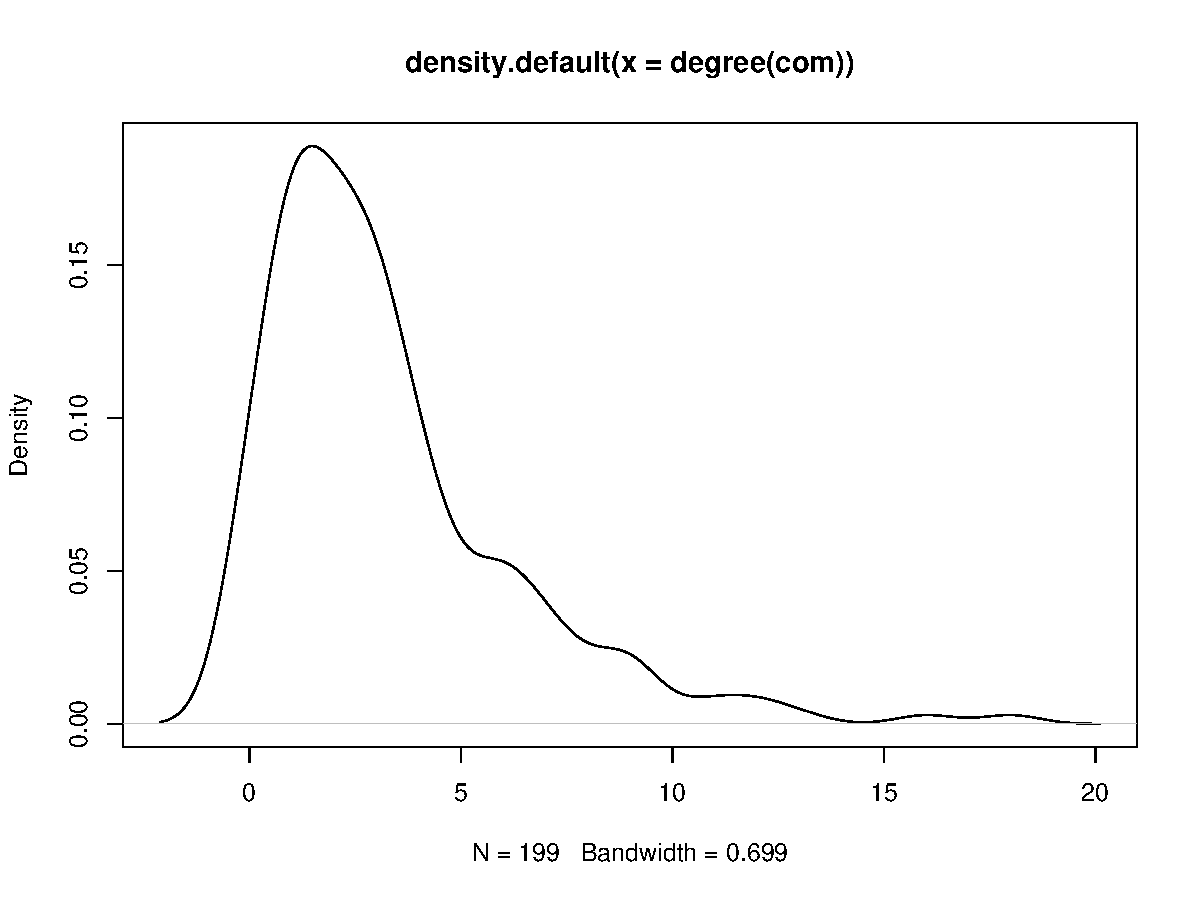
\includegraphics[height=.2\textheight, clip=true, trim=1cm 1cm 0cm 2cm]{figures/deg_com.pdf} & 
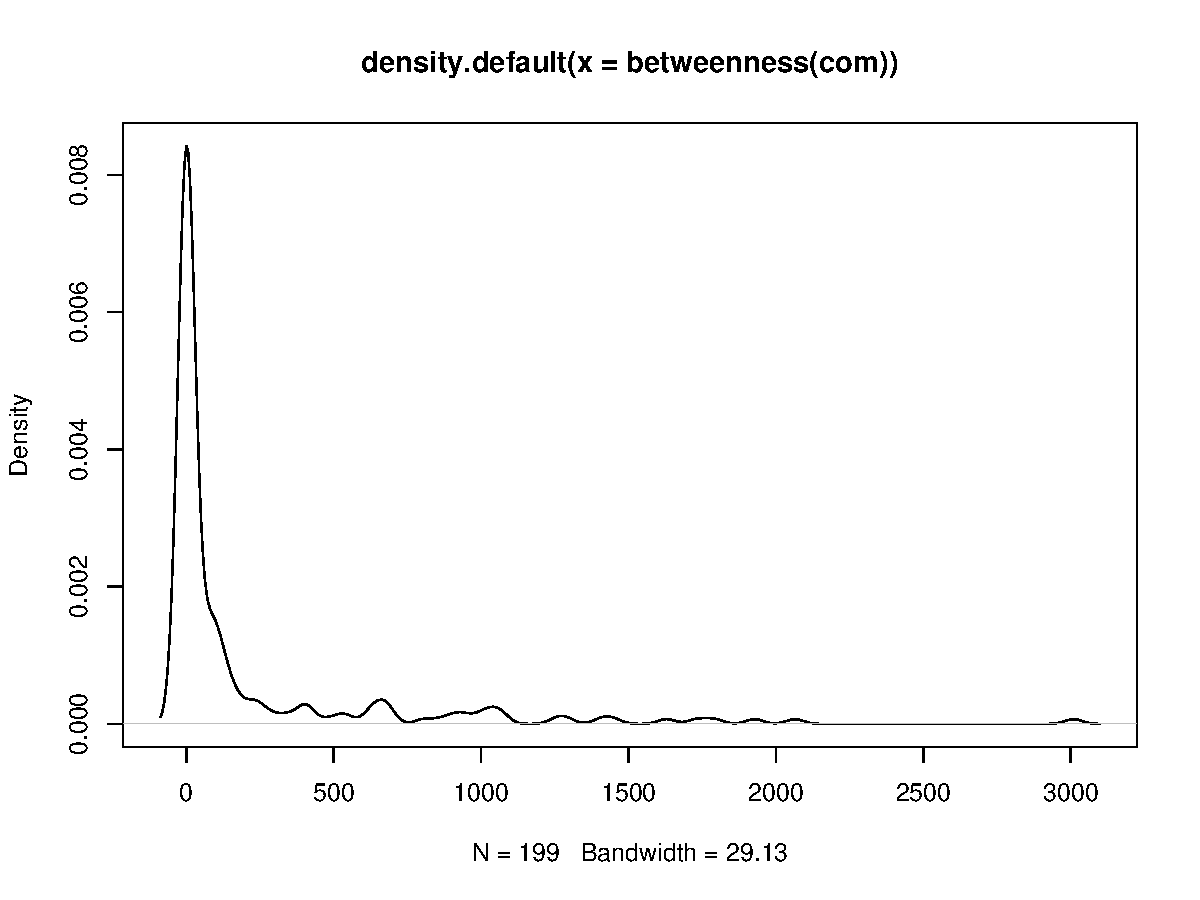
\includegraphics[height=.2\textheight, clip=true, trim=1cm 1cm 0cm 2cm]{figures/cen_com.pdf} \\ 

Social & Social\\
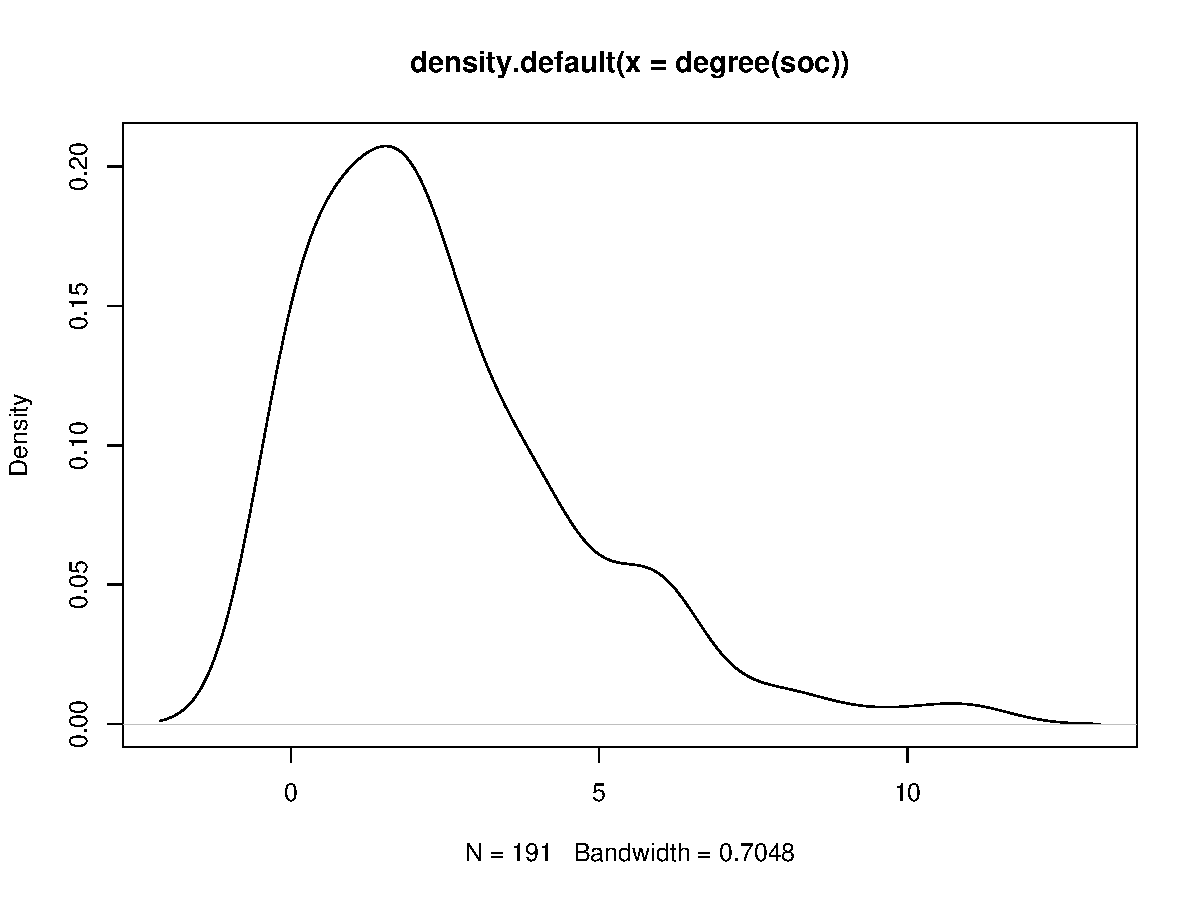
\includegraphics[height=.2\textheight, clip=true, trim=1cm 1cm 0cm 2cm]{figures/deg_soc.pdf}  &
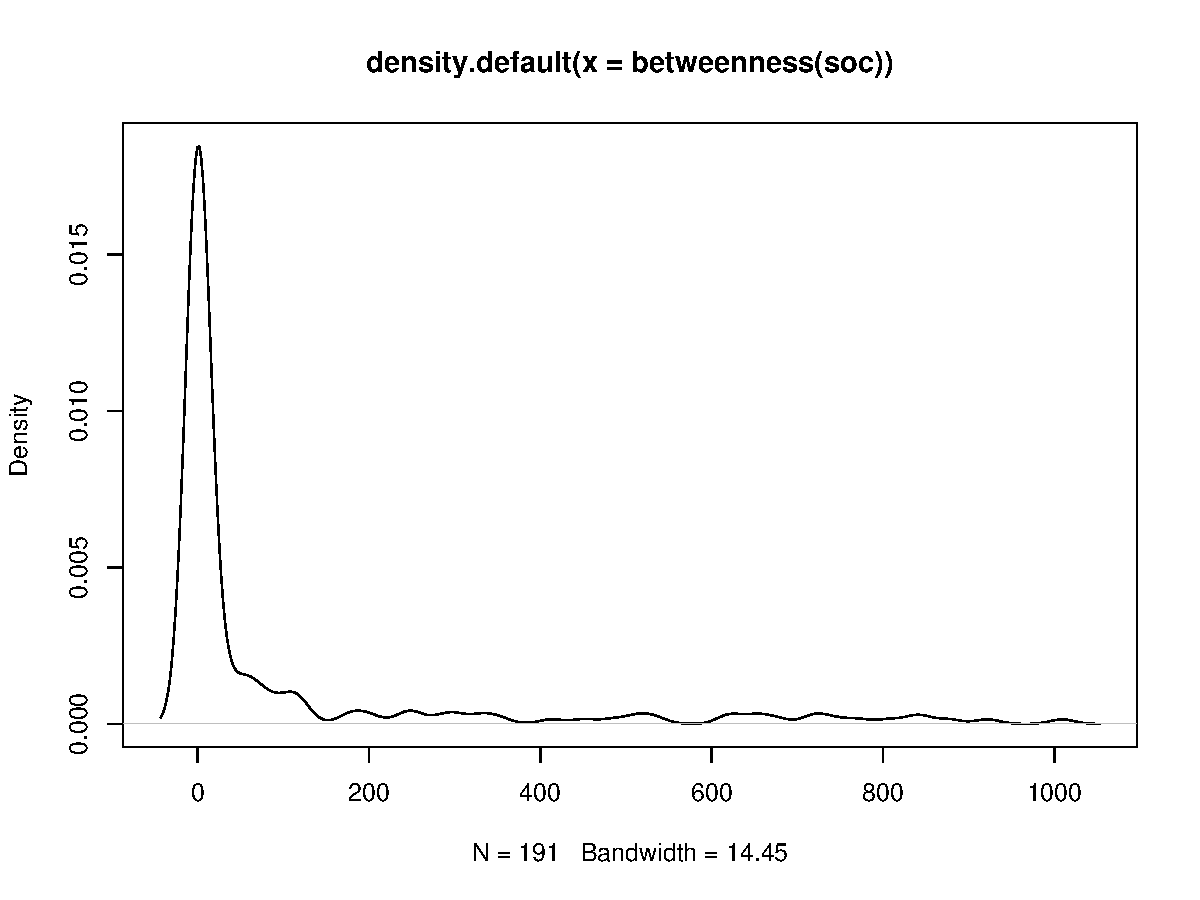
\includegraphics[height=.2\textheight, clip=true, trim=1cm 1cm 0cm 2cm]{figures/cen_soc.pdf}\\

Info Exchange & Info Exchange\\

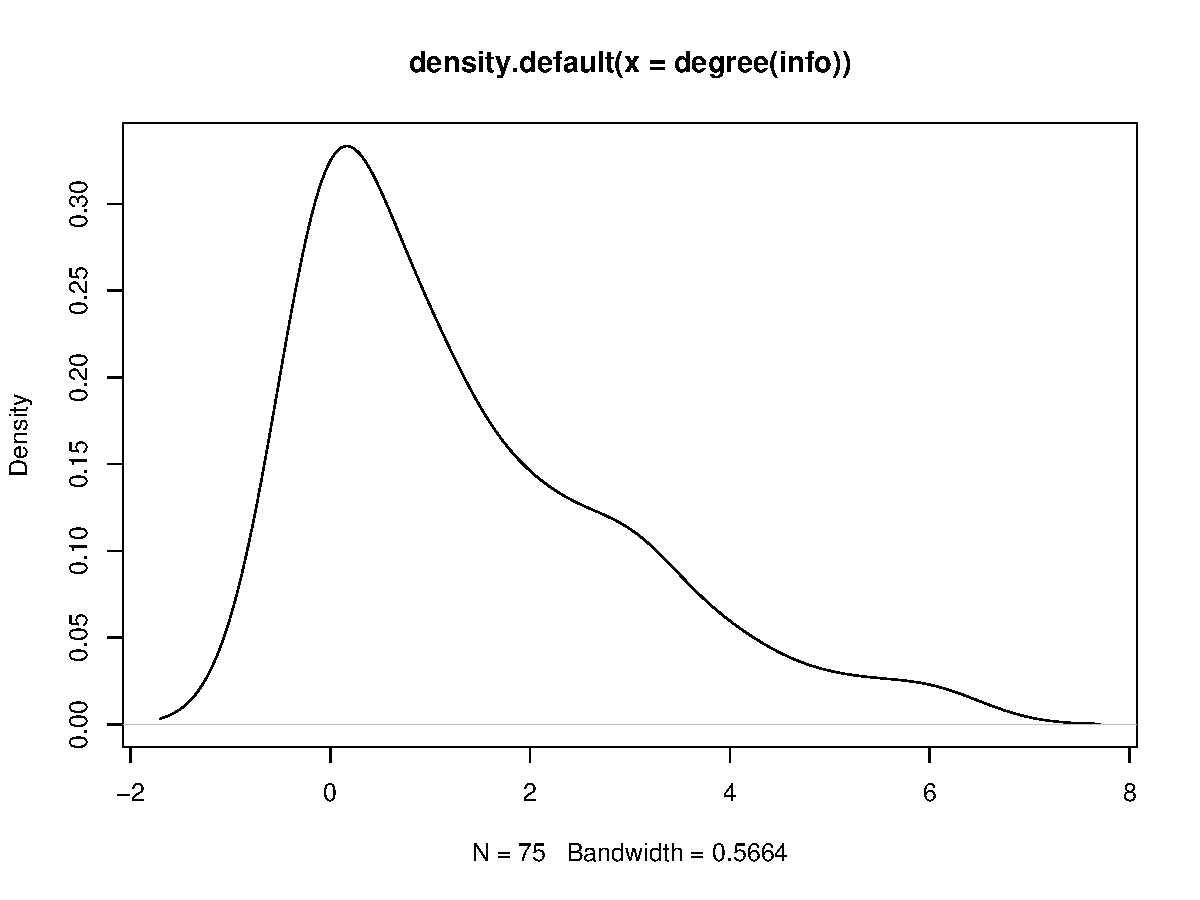
\includegraphics[height=.2\textheight, clip=true, trim=1cm 1cm 0cm 2cm]{figures/deg_info.pdf} &
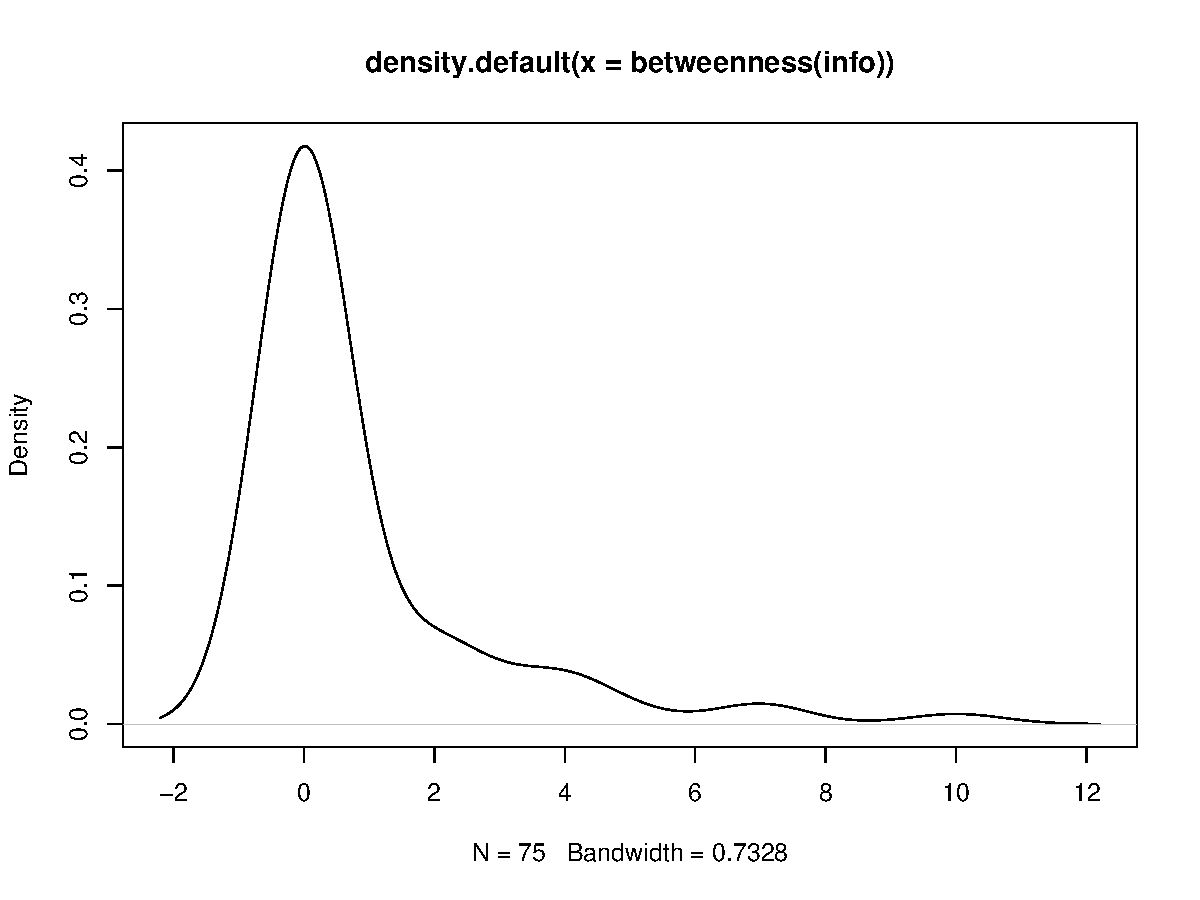
\includegraphics[height=.2\textheight, clip=true, trim=1cm 1cm 0cm 2cm]{figures/cen_info.pdf} \\
\caption{\label{fig:SS_plots} Density plots for degree distribution and betweenness centrality for all three networks.}
\end{longtable}
\end{figure}


\begin{table}[!htbp] \centering
  \caption{Summary Statistics: Networks}
  \label{SS_DV}
\begin{tabular}{@{\extracolsep{5pt}} lccccc}
\\[-1.8ex]\hline
\hline \\[-1.8ex]
Network & Measurement & Value  \\
\hline \\[-1.8ex]
Communication& Edge Density & $0.008$ \\
Communication& Reciprocity  & $0.255$ \\
Communication& Transitivity  & $0.108$ \\
\hline \\[-1.8ex]

Social& Edge Density & $0.006$ \\
Social& Reciprocity  & $0.203$ \\
Social& Transitivity  & $0.119$ \\
\hline \\[-1.8ex]

Info Exchange& Edge Density & $0.009$ \\
Info Exchange& Reciprocity  & $0.157$ \\
Info Exchange& Transitivity  & $ 0.135$ \\
\\[-1.8ex]\hline
\hline \\[-1.8ex]
\end{tabular}
\end{table}






\begin{table}[!htbp] \centering
  \caption{Summary Statistics: Independent Variables}
  \label{SS_IV}
\begin{tabular}{@{\extracolsep{5pt}} lccc}
\\[-1.8ex]\hline
\hline \\[-1.8ex]
 &  \multicolumn{3}{c}{Proportion} \\
\hline \\[-1.8ex]
Variable & Communication & Social & Info Exchange\\
\hline \\[-1.8ex]

Same Education Level  & $71\%$ & $70\%$ & $74\%$\\
Same Floor  & $10\%$ & $10\%$ & $12\%$\\
Both Leadership & $6\%$ & $7\%$ & $6\%$\\
Both non-Leadership & $10\%$ & $10\%$ & $14\%$\\
Same State  & $10\%$ & $9\%$ & $12\%$\\
Same Party & $46\%$ & $50\%$ & $43\%$\\
\hline \\[-1.8ex]
 &  \multicolumn{3}{c}{Average} \\
\hline \\[-1.8ex]
$\Delta$ Age & $12$ & $12$ & $13$\\
\\[-1.8ex]\hline
\hline \\[-1.8ex]
\end{tabular}

\end{table}


\subsection{Hypotheses}


The main hypothesis of the paper is that political parties actively work to form ties among members and thus counter the individualistic tendencies of politicians to increase their own electoral share/power at the expense of the party. The network then creates trust and cohesion among the actors, while also facilitating monitoring. The author expects that this will the the stronger driver of the tie formation, rather than individual traits. 

The secondary hypothesis of the paper are is that similar individual traits drive network ties, even if less so than party membership. The author includes five different traits. The first is that when politicians are both in leadership positions they will need to interact more, but when neither are in leadership positions they will not need to interact with one another and can rely on party leaders. The second is that when politicians have similar ages they will form connections based on shared experiences.  The third is that when politicians are from the same state they will form connections since there is a proportional voting system in Brazil and that means that coordination among members in the same states is necessary to exchange information about what the local needs are. The fourth is that politicians with the same education level are likely to have similar knowledge and social class, which increases the chance of network ties. The fifth is that when politicians work on the same floor this creates opportunity for interaction.


\subsection{Replication design}

The ERGMs are specified in the article to include a intercept term, the exogenous covariates, and a term for transitive ties. Transitive ties is a network statistic, specific to network models and is defined as the change in the likelihood of a tie between two nodes given the presence of a two-path or a triad closure. A two-path between nodes $i$ and $j$ is defined as node $i$ having a directed edge path to node $k$ and node $k$ having a directed edge to node $j$, or put differently, there exists a connection between the nodes with only two edges.
 

For the LSMs, the specification is the same except it does not include the include a transitive ties term. This is because the model does not have network statistics as an ERGM model does, but instead we specify the latent space that models higher order dependences, which would include transitivity. For our extensions we use the euclidean distance model term that is equal to the negative euclidean distance between actors in the unobserved social space. We estimated the term along two dimensions and across two or three clusters, depending on best model fit using the BIC. The SBMs do not include a constant term as the block or group effect takes the place of the intercept term. It also does not have network terms like transitive ties as it accounts for dependencies using the latent space along a multinomial distribution to determine block membership for the nodes. 


\subsection{Results}


The results from the LSMs indicate that the latent space explains less of the variation in the ties than the network statistics in ERGMs, as the coefficients for exogenous covariates, while signed the same, are mostly larger in magnitude. One exception is the node-match variables for leadership, where in Model 1 the effect size is slightly larger, but in Model 3 the effect size is nearly one-third smaller. Also, the changes in magnitude are generally smaller for the leadership variables than the other variables. The latent space plots (Table \ref{fig:LSM_plot_1}) show that the clusters are not distinct from one another, but rather there are inside groups that form clusters and each subsequent group are nodes that are less central to the graph.

The results from the SBMs indicate that the latent space and block membership explains more of the variation in the ties than the network statistics in ERGMs, as the coefficients for exogenous covariates, while signed the same, are mostly smaller in magnitude. Also, the coefficient estimates have smaller standard errors relative to the size of the estimate. In Table \ref{fig:SBM_plot_1} block likelihoods for each node assignment shows that for communication ties in Model 1, we see that the blocks are fairly evenly distributed, but that membership not predominant and that many of the nodes have spread out likelihoods for membership assignment. In Model 2 we see that this shared membership is even greater for the social networks. However, for the information network in Model 3, membership likelihood is sharply separated and concentrated in one block for each node.

It is not immediately obvious which model performs best for this application. In general there are a couple factors that influence which model is used for final analysis. This first is that theory should drive the decision of which model to use. For example, if a scholar is interested in studying the presence and magnitude of a specific type of network dependence, the ERGM is the best suited model for this. While software does allow terms such as transitive ties to be estimated in LSMs, current methods rely on psuedo-likelihood estimation and this approach has net yet been well vetted. Additionally, if a scholar is interested in understanding relationships between clusters of observations and the likelihood that an actor in one cluster will form ties with an actor in another cluster, the SBM is best suited for examining this. The second issue is practicality. Any scholar that has used ERGMs, has likely dealt with model degeneracy. For this reason, and if the scholar wants to account for network dependence, but does not want to work through specifying relevant dependence terms, especially those limited due to software limitations, the LSM is a viable option. Additionally, there are times data characteristics drive decisions. For example, if a network has a high number of zeroes, scholars that do not want to write their own software will need to chose software that implements model specification that  best accounts for zero-inflation. However, as the replication has shown, the flexibility of the of each method often makes it possible that if for nothing but robustness testing, scholars can implement more than one model type and even gain insight through comparing model results. 


\begin{landscape}
\begin{table}[!htbp] \centering
\caption{Replication Results}
\label{table:coefficients}
\begin{tabular}{lccccccccc}
\\[-1.8ex]\hline
\hline \\[-1.8ex]
 & ERGM & LSM & SBM  & ERGM & LSM & SBM & ERGM & LSM & SBM\\
\hline \\[-1.8ex]
 &  \multicolumn{3}{c}{Communication Networks} &  
 \multicolumn{3}{c}{Social Networks}&  
 \multicolumn{3}{c}{Information Exchange}\\
\hline
Edges (intercept)   & $-$5.67$^{***}$ &$-3.10^{***}$ & - - & 
$-$6.07$^{***}$ &$-3.00^{***}$& - - & 
$-$5.74$^{***}$ &   $-3.12^{***}$  & - -  
\\ 
& (0.16) & (0.09) & - - &(0.19) & (0.29) &  - - &(0.45) & (0.62)& - -
 \\ 
  & & & \\ 
$\Delta$ Age & $-$0.02$^{***}$ & $-0.03^{***}$  & $-$0.01$^{***}$ &
$-$0.02$^{***}$ & $-0.04^{***}$    &$-$0.01$^{***}$ &
 $-$0.06$^{***}$ & $-0.08^{***}$  &   $-$-0.04$^{***}$ \\
  & (0.01)   & (0.01) & ($<$0.01) &
  (0.01) & (0.01) &  ($<$0.01) &
  (0.02)& (0.03)  &(0.01)\\ 
  & & & \\ 
Same Education Level & 0.164 & $0.22^{***}$ & 0.143$^{**}$&
0.161 & $0.35^{***}$ & 0.081 &
0.600$^{*}$ &  $0.93^{**}$ & 0.293$^{**}$ \\ 
  & (0.125) &(0.031) & (0.057) &
  (0.144) & (0.084) &  (0.070) &
  (0.334) &(0.433)&(0.150)\\ 
  & & & \\ 
Same Floor & 0.76$^{***}$ & $1.02^{***}$  & 0.32$^{***}$ & 
1.37$^{***}$      & $1.53^{***}$   &   0.63$^{***}$   &
0.79$^{**}$ & $1.16^{**}$  & 0.43$^{**}$ \\ 
  & (0.15)  & (0.15) & (0.07) &
  (0.14) & (0.01) &  (0.07) & 
  (0.39)& (0.49) &(0.17) \\ 
  & & & \\ 
Both non-leadership & $-$0.66$^{***}$ &   $-0.82^{***}$   & $-$0.28$^{***}$ &           
$-$0.24$^{*}$ &$-0.28^{**}$& $-$0.13$^{**}$& 
$-$0.81$^{**}$ & $-0.82^{**}$  & $-$0.41$^{***}$\\
  & (0.13) & (0.05) & (0.05) & (0.14) &  (0.42) & (0.06)&(0.34)   & (0.11)& (0.14)\\ 
  & & & \\ 
Both leadership & 0.534$^{***}$ &  $0.61^{***}$     &0.21$^{***}$ &    
0.47$^{**}$ &   $0.44$   &0.20$^{**}$ & 
0.84$^{**}$ & $0.64$&0.34$^{**}$ \\ 
  & (0.16) & (0.01)&  (0.07) & 
  (0.21) & (0.30)& (0.10)  &
  (0.40)   & (0.5)& (0.17)
    \\ 
  & & & \\ 
Same State & 2.12$^{***}$ &$2.75^{***}$& 1.05$^{***}$ &
2.11$^{***}$ &$2.56^{***}$ &1.04$^{***}$ & 
0.99$^{**}$ &$1.31^{*}$& 0.46$^{**}$\\ 
  & (0.12) &(0.11)& (0.06) &
  (0.14) &(0.18)& (0.07) &
  (0.43) &(0.67)& (0.20)\\ 
      \\ 
  & & & \\ 
Same Party & 2.32$^{***}$ &$2.86^{***}$ & 1.09$^{***}$ & 
2.05$^{***}$ &$2.30^{***}$& 0.99$^{***}$&
2.96$^{***}$ &$3.47^{***}$&1.36$^{***}$\\ 
  & (0.12) &(0.11)& (0.05) &
   (0.14) &(0.03)& (0.07)&
   (0.34) &(0.41)& (0.14) \\
  & & & \\ 
 Transitive ties & 0.66$^{***}$ &- - &- -& 0.90$^{***}$ &- -&- -&0.57&- -& - -\\ 
  & (0.12) &- - &- -& (0.14) &- - &- -& (0.40)&- - &- - \\ 
  & & & \\ 
\hline \\[-1.8ex] 
Latent Dimensions & - - & 2 & - - & - - & 2 & - - & - - & 2 &- -\\
$n$ Blocks/Clusters & - - & 3 & 3 & - - & 3 & 2 & - - & 2 & 3\\
$N$ & 39,402  & 39,402 &  39,402 &36,290 &36,290 &  36,290 &5550& 5550&  5550\\  
\hline
\multicolumn{4}{l}{\scriptsize{Note: {$^{*}$p$<$0.1; $^{**}$p$<$0.05; $^{***}$p$<$0.01}}}
\end{tabular}
\end{table}
\end{landscape}


\begin{longtable}[!h]{ccc}
Model 1 & Model 2 & Model 3\\
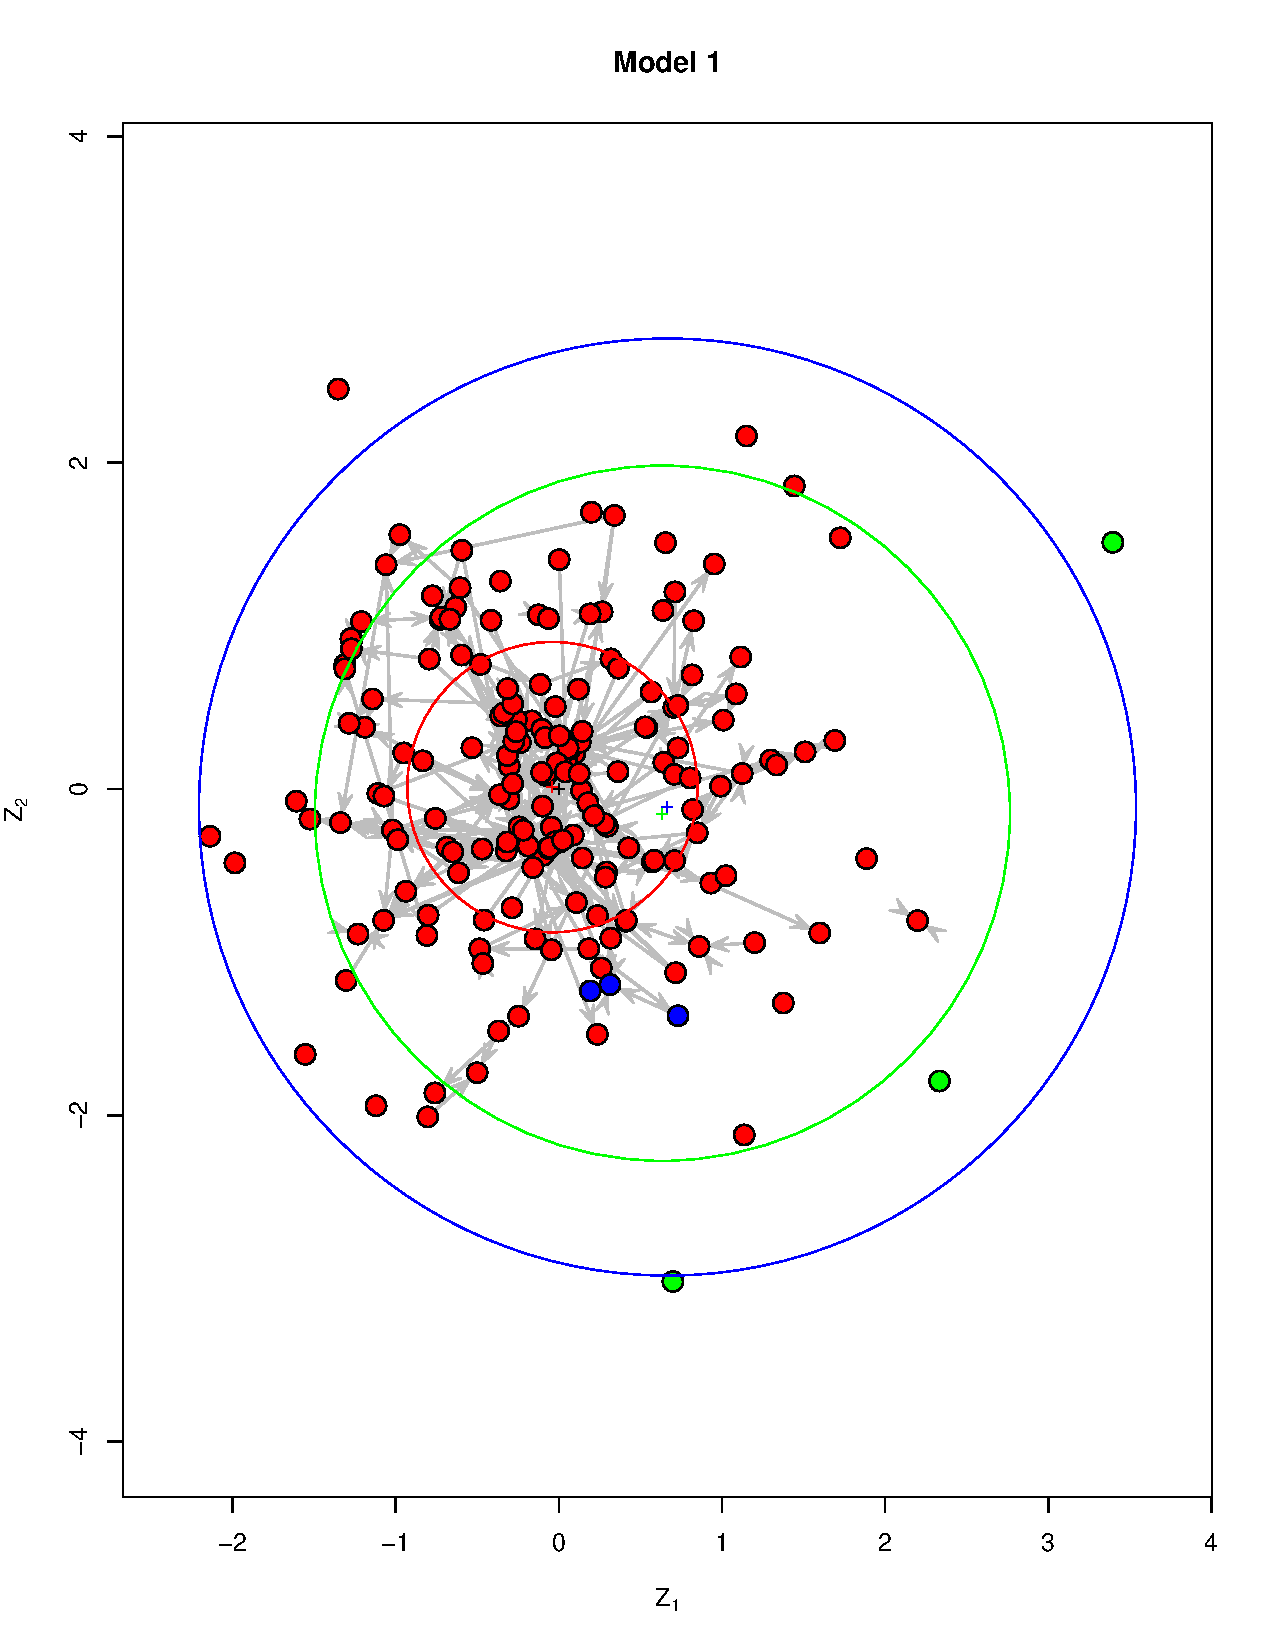
\includegraphics[height=.3\textheight, clip=true, trim=2.06cm 2.55cm 1cm 2cm]{figures/LSM_m1.pdf}   & 
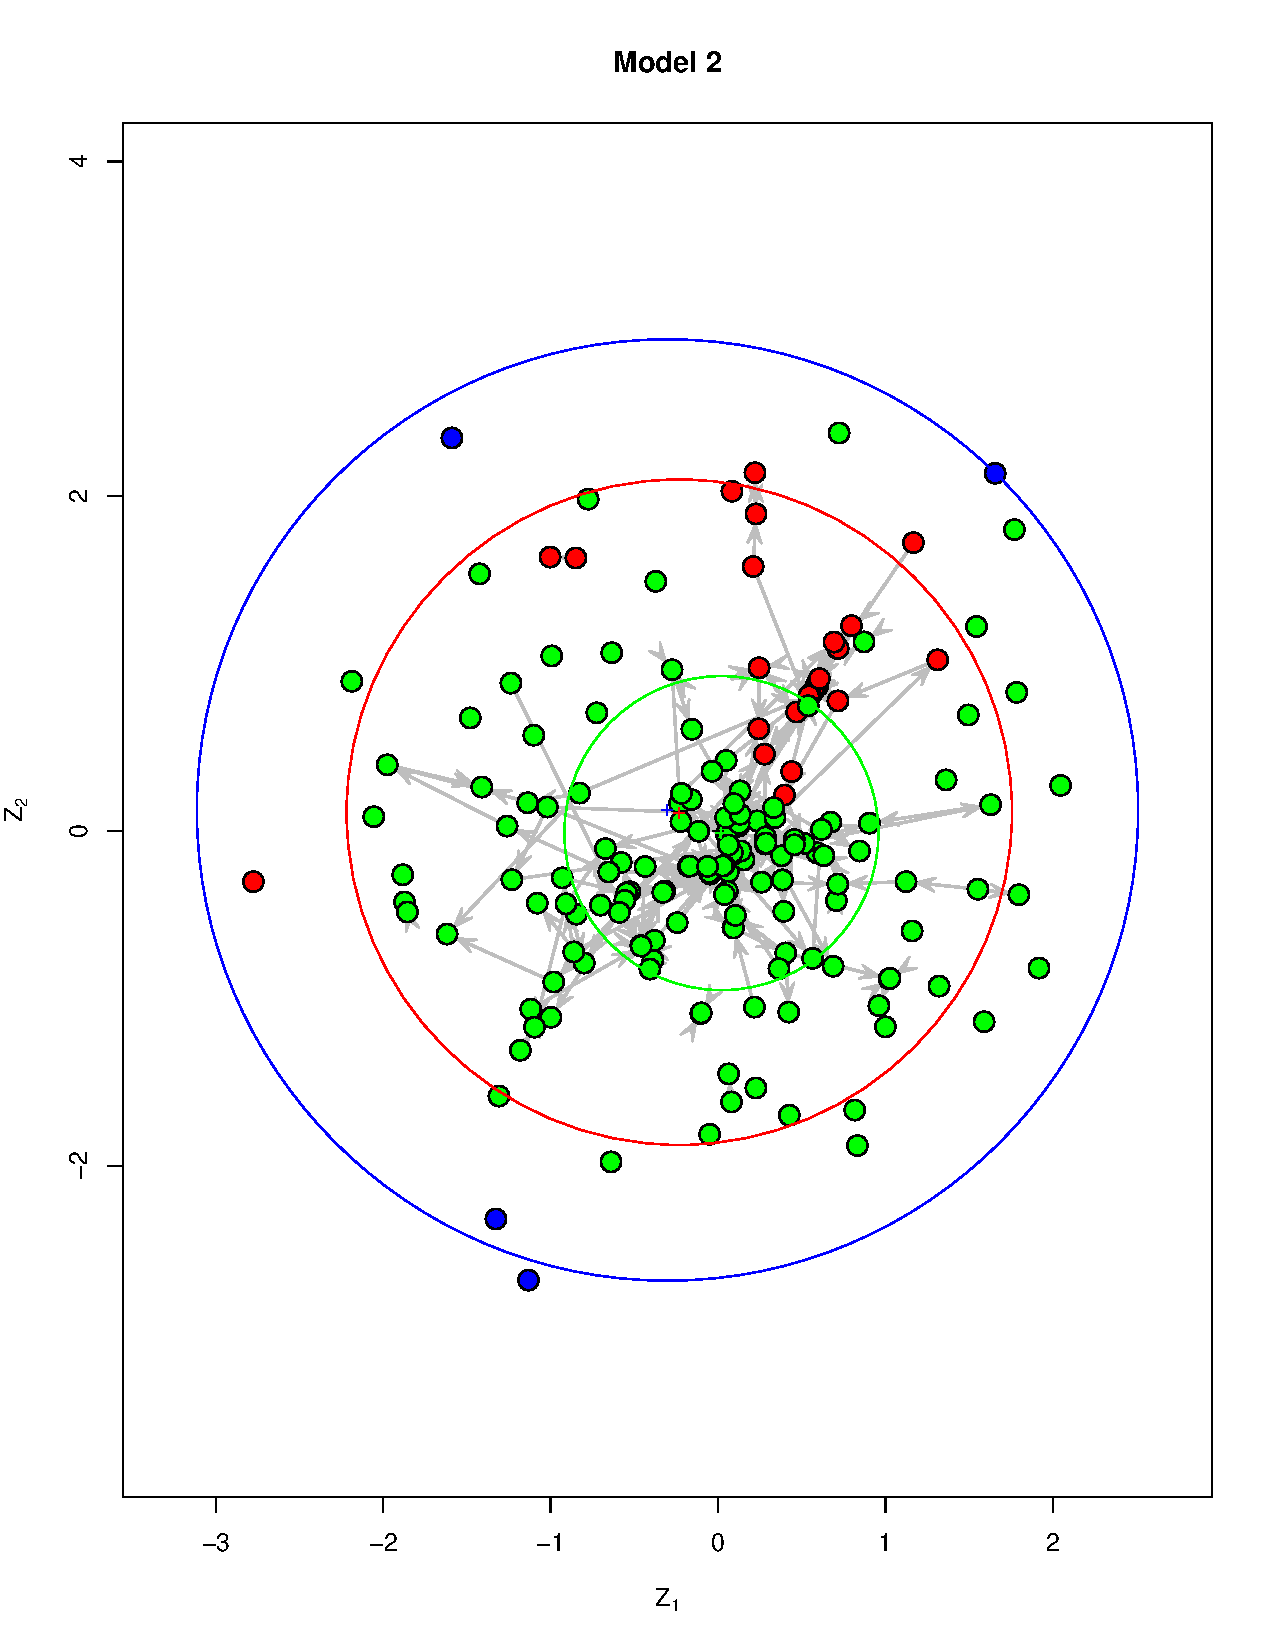
\includegraphics[height=.3\textheight, clip=true, trim=2.05cm 2.55cm 1cm 2cm]{figures/LSM_m2.pdf}  
&
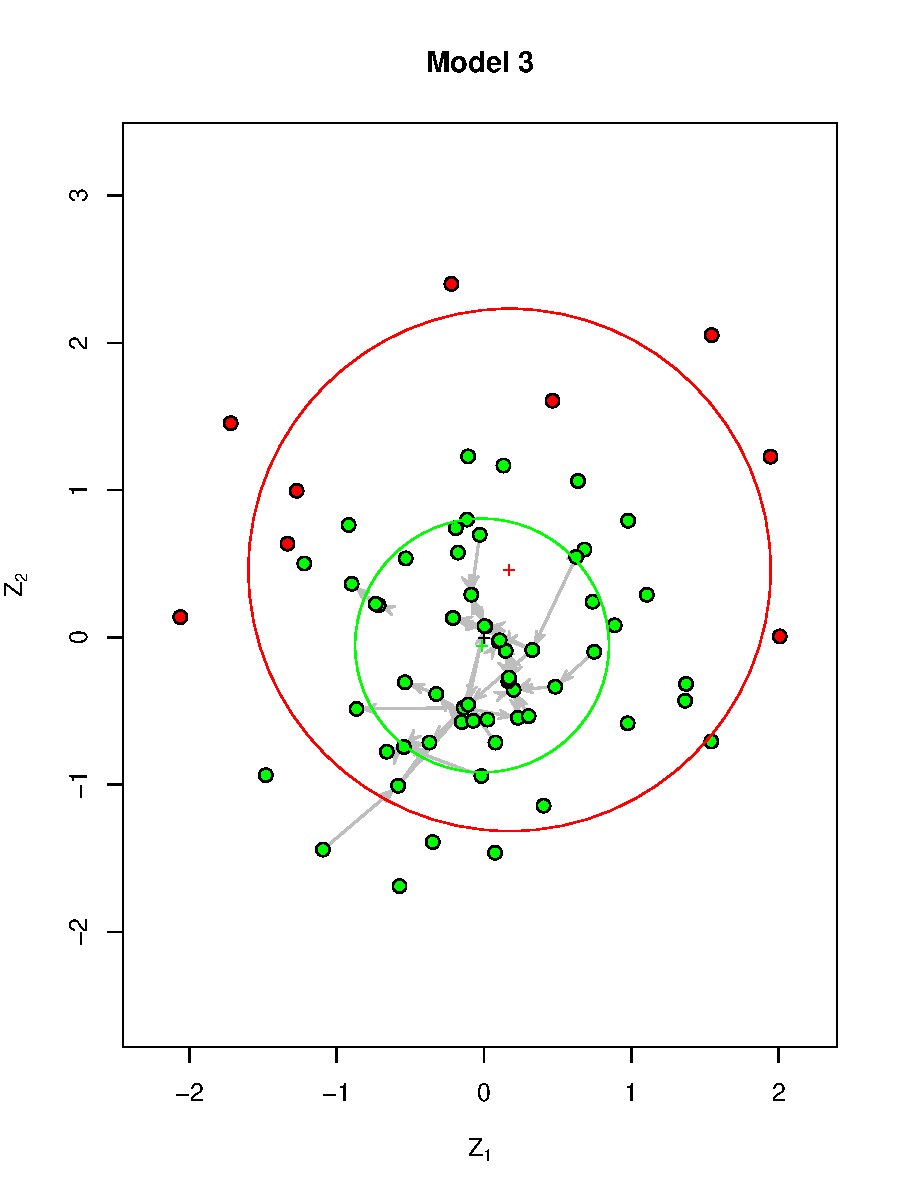
\includegraphics[height=.3\textheight, clip=true, trim=2.05cm 2.55cm 1cm 2cm]{figures/LSM_m3.pdf} \\
\caption{\label{fig:LSM_plot_1} Plots of latent space positions for the LSMs along two dimensions. The gray lines represent the directed edges between nodes. Each cluster has a unique color that is used for the node color and line that encloses the cluster.}
\end{longtable}

\clearpage
\begin{longtable}[!h]{c@{\hskip 0cm}c}
Model 1 \\
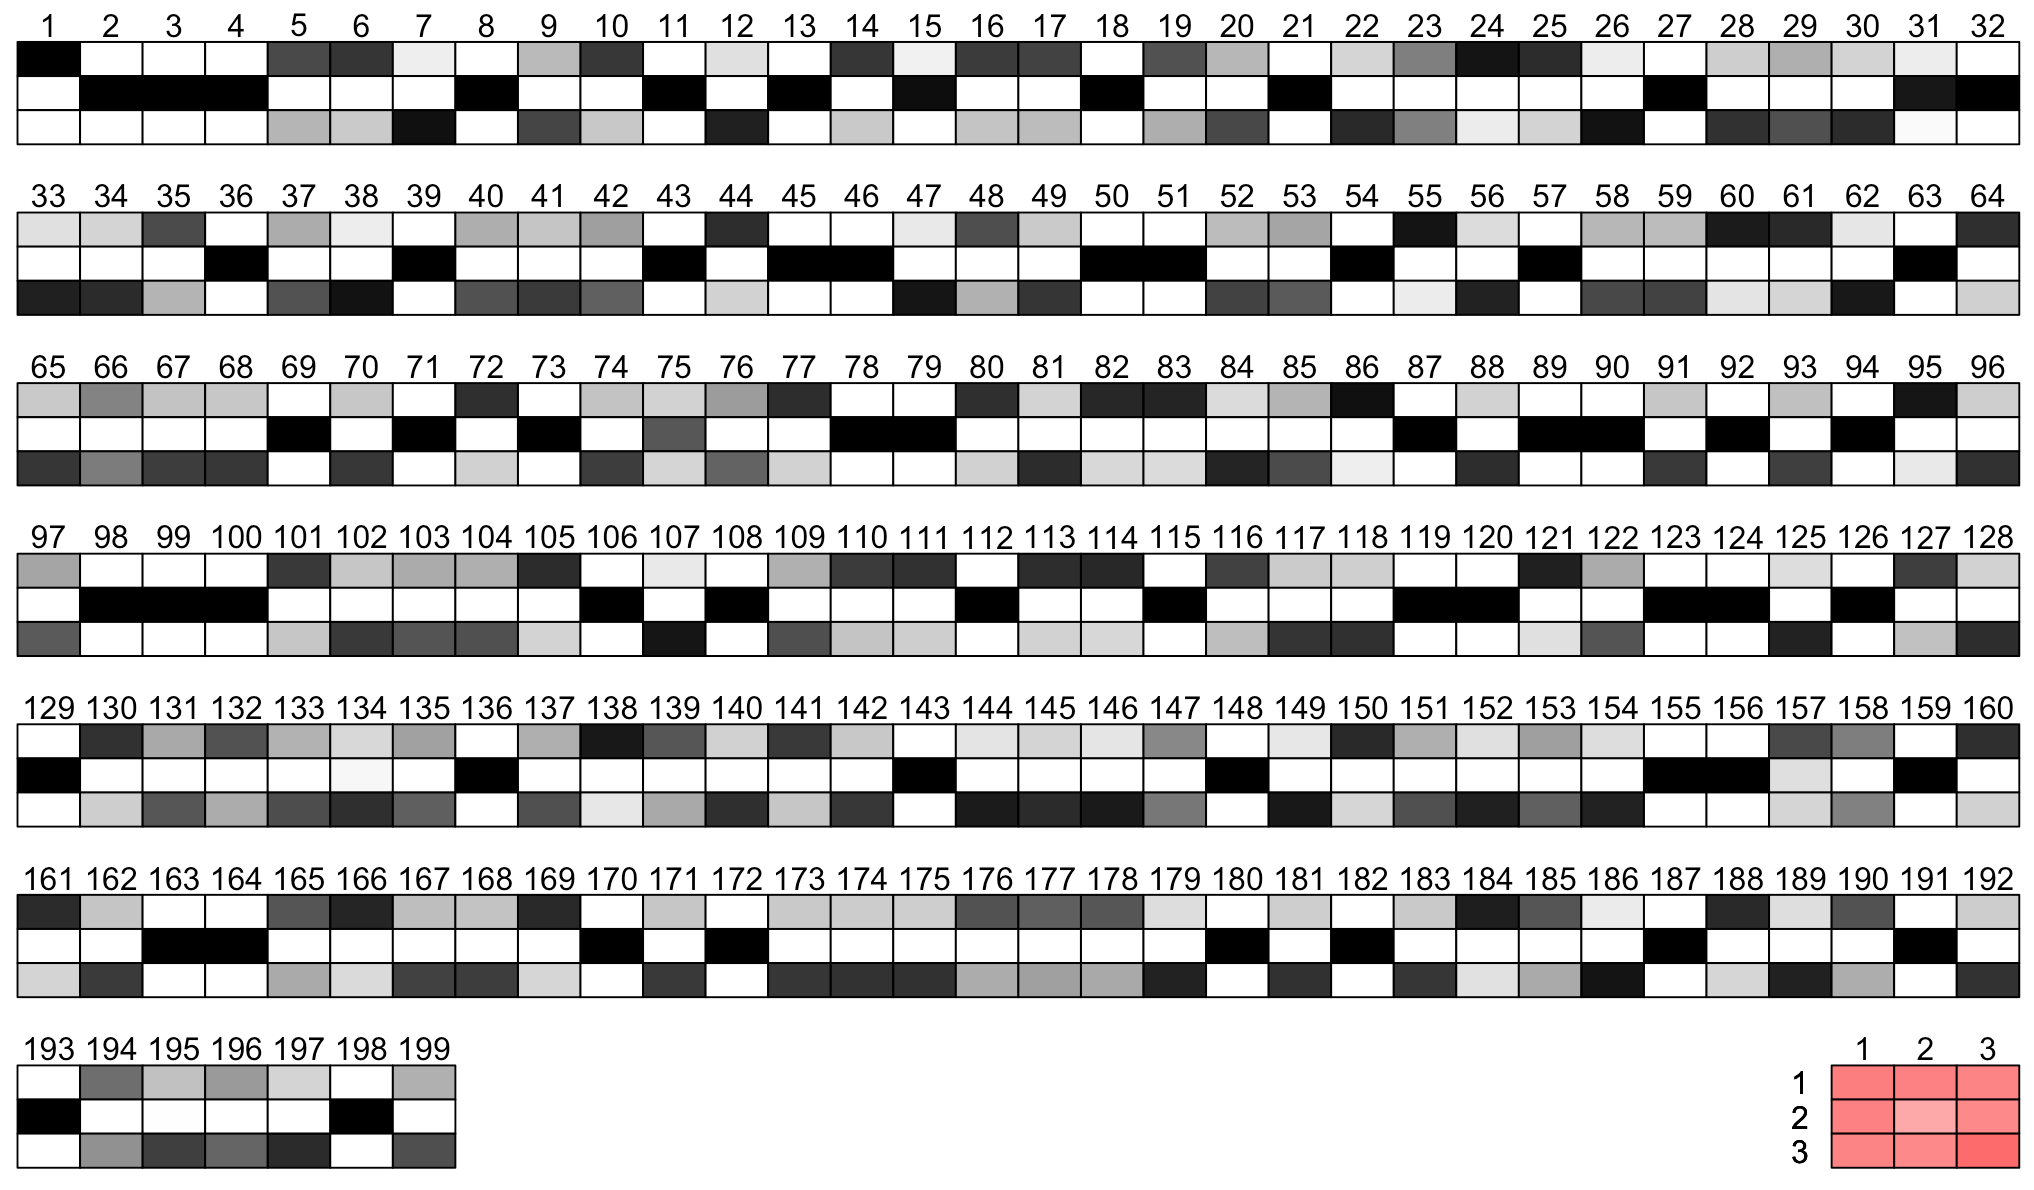
\includegraphics[height=.26\textheight, clip=true, trim=0cm .25cm 0cm 0cm]{figures/SBM_m1}   \\
Model 2 \\
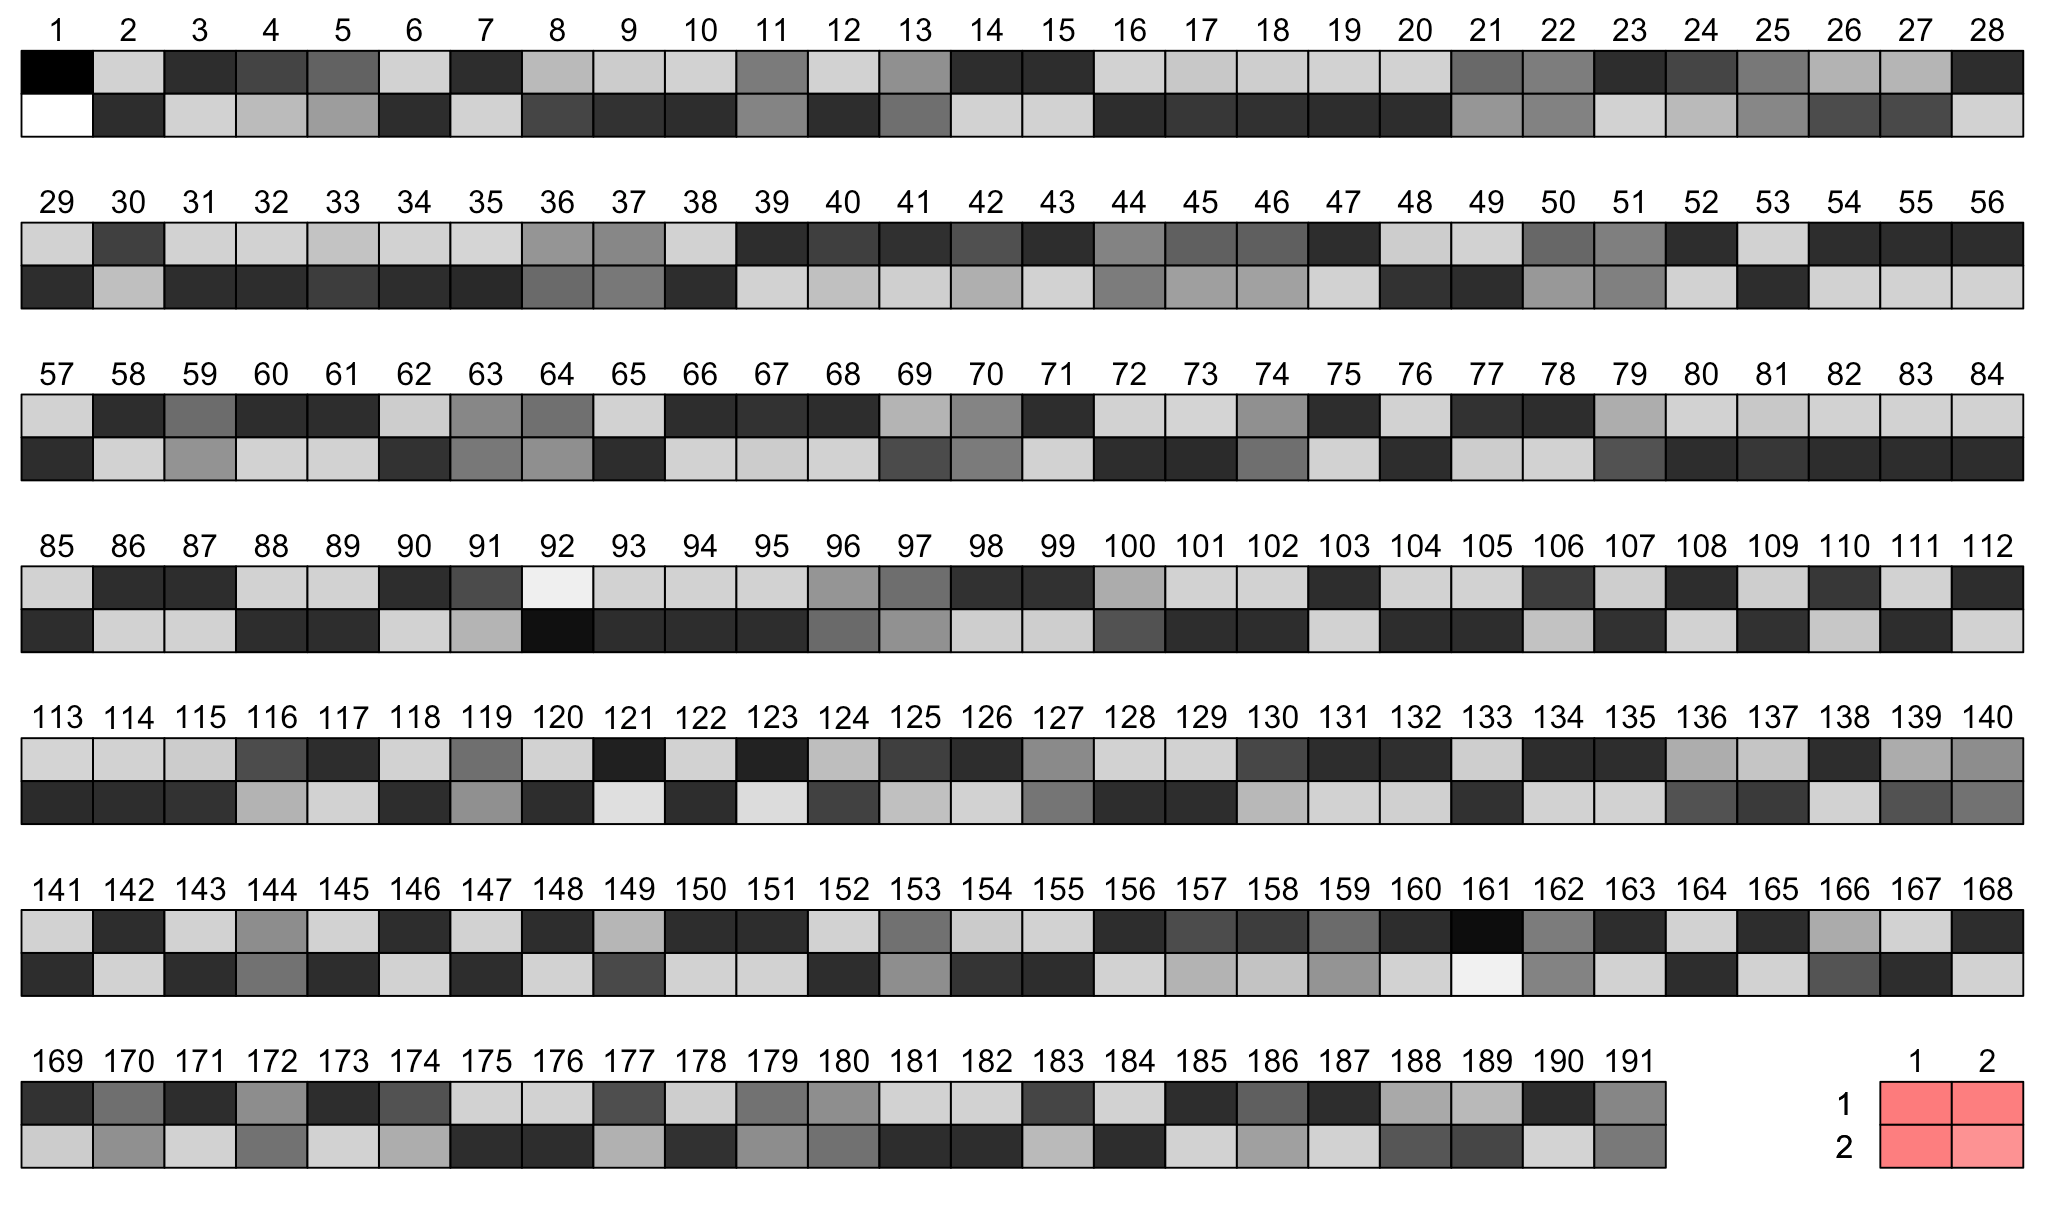
\includegraphics[height=.26\textheight, clip=true, trim=0cm 0cm 0cm 0cm]{figures/SBM_m2}   \\
Model 3 \\
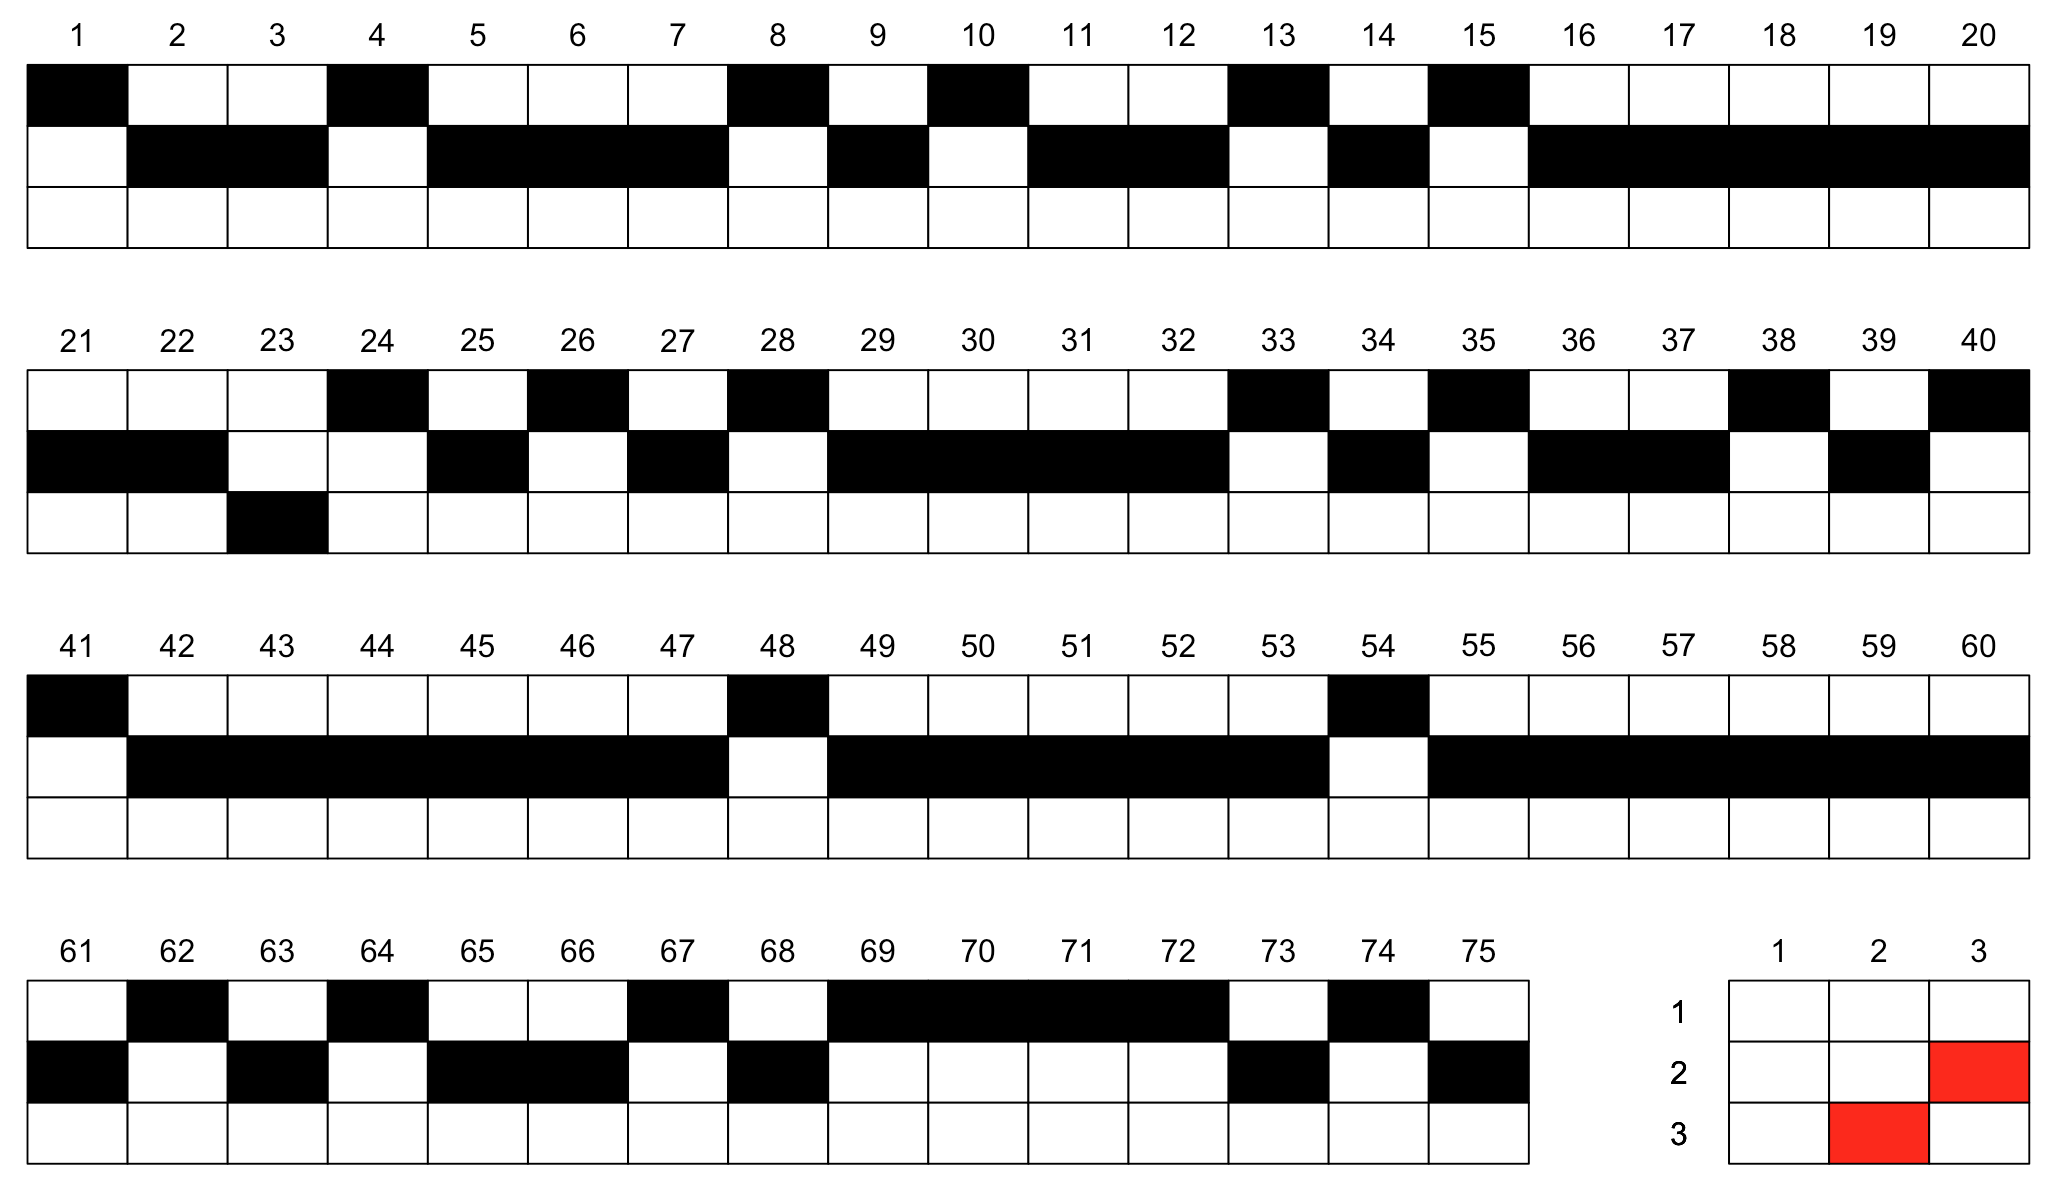
\includegraphics[height=.26\textheight, clip=true, trim=0cm 0cm 0cm 0cm]{figures/SBM_m3}   \\
\caption{\label{fig:SBM_plot_1} SBM block assignment plots. Each column represents one node and the rows are the block possibilities for each node. The blocks are shaded from white to black for the probability of block membership, with white representing a probability of approximately zero and black representing a likelihood of approximately one. The bottom right box is shaded according to the value of the block matrix value.}
\end{longtable}


\section{Discussion}


Advances in methodology and software availability has allowed inferential network analysis to increasingly be used in political science. Ever increasing availability of computational power, has made these models that rely on computationally intensive Bayesian estimation methods easier to implement and apply to networks that number in the millions of nodes. With the inherent relational structure of international relations data, inferential network analysis will continue to make an impact in political science methodology and substantive discourse as a tool that allows researchers to study the many networks present in political science research agendas, while accounting for and better understanding the relational structure of the data. 

We hope that this chapter will help guide scholars in using available network tools and understanding the methodology behind them, as well a their usefulness and their limitations. In this chapter we have reviewed three of the most commonly used statistical network models, but it should be noted that other models such as the stochastic actor oriented model are available and have been used in political science. We would also like to emphasize that there is not a consensus for which model is best for network analysis in political science and it likely that scholars will need to continue to weigh the pros and cons of each model for their specific application. As for the application, it provides a brief overview of network descriptive statistics and model specification options, but it should be noted that there many other useful network descriptive measures that scholars can employ, as well as other dependence terms to include in model specification, especially when using the ERGM. Also, while \R is increasingly the software of choice for inferential network analysis in political science and contains a vast library of packages for static, time-dependent, and weighted networks, other options include the \textsf{Python} library \texttt{NetworkX} or user friendly GUI based software like \textsf{PNet} and \textsf{UCINET}. 






\clearpage

\bibliographystyle{apsr}
\bibliography{bibliography}




\end{document}